\chapter{Problem Statement}
\todo[inline]{Todo: Expand everything in this section}
The thesis will focus on parliamentary proceedings from the German
\emph{Bundestag}. These proceedings are available online as PDF files dating
back to 1949, and have used essentially the same document layout and conventions
since the start. Semantically, the layout of these documents forms a shallow
tree:
\begin{center}
  \begin{forest}
    [root
      [topic
        [speech]
        [\dots]
        [speech]
      ]
      [\dots]
      [topic
        [speech]
        [\dots]
        [speech]
      ]
    ]
  \end{forest}
\end{center}
Each document consists of a series of topics to discuss, where each topic
contains a series of speeches made by the present politicians. The task to be
solved is retrieving these speeches as accurately and robustly as possible.
Luckily, in this case a rule-based system for segmenting the files already
exists and was used to create a fairly large training set. Since in general such
a system will not exist and annotating the data by hand is expensive, a big
focus is on limiting the amount of required training data as much as possible.

\begin{figure}[htbp]
  \centering
  \begin{subfigure}[b]{0.6\textwidth} 
    \centering
    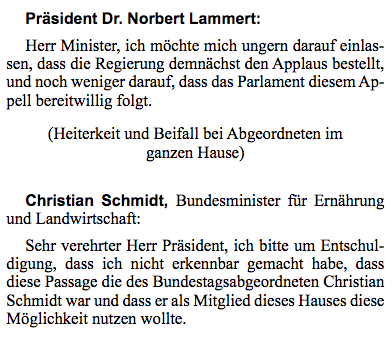
\includegraphics[width=\textwidth]{figures/source.png}
    \caption{The source PDF}
  \end{subfigure}
  \vspace{0.10\textwidth}
  \begin{subfigure}[b]{\textwidth}
	\centering
    \begin{lstlisting}[language=xml, morekeywords={text}]
      <text top="122" left="125" width="143" height="16" font="3">
          <b>Dr. Norbert Lammert </b>
      </text>
      <text top="122" left="269" width="83" height="17" font="4">
          (CDU/CSU):
      </text>
      <text top="142" left="125" width="328" height="17" font="4">
          Herr Alterspräsident, lieber Kollege Riesenhuber, ich
      </text>
      <text top="158" left="108" width="156" height="17" font="4">
          nehme die Wahl gerne an.
      </text>
      <text top="186" left="141" width="278" height="17" font="4">
          (Beifall im ganzen Hause – Abgeordnete aller
      </text>
      <text top="203" left="158" width="242" height="17" font="4">
          Fraktionen gratulieren dem Präsidenten)
      </text>
    \end{lstlisting}
    \caption{XML}
  \end{subfigure}
  \caption{The data representations}
  \label{fig:example}
\end{figure}

The dataset, obtained through a rule-based system as described in the
introduction, is currently complete dating back to 2005. It features 811
documents, containing 43.252 speeches.

\begin{figure}[htbp]
  \centering
  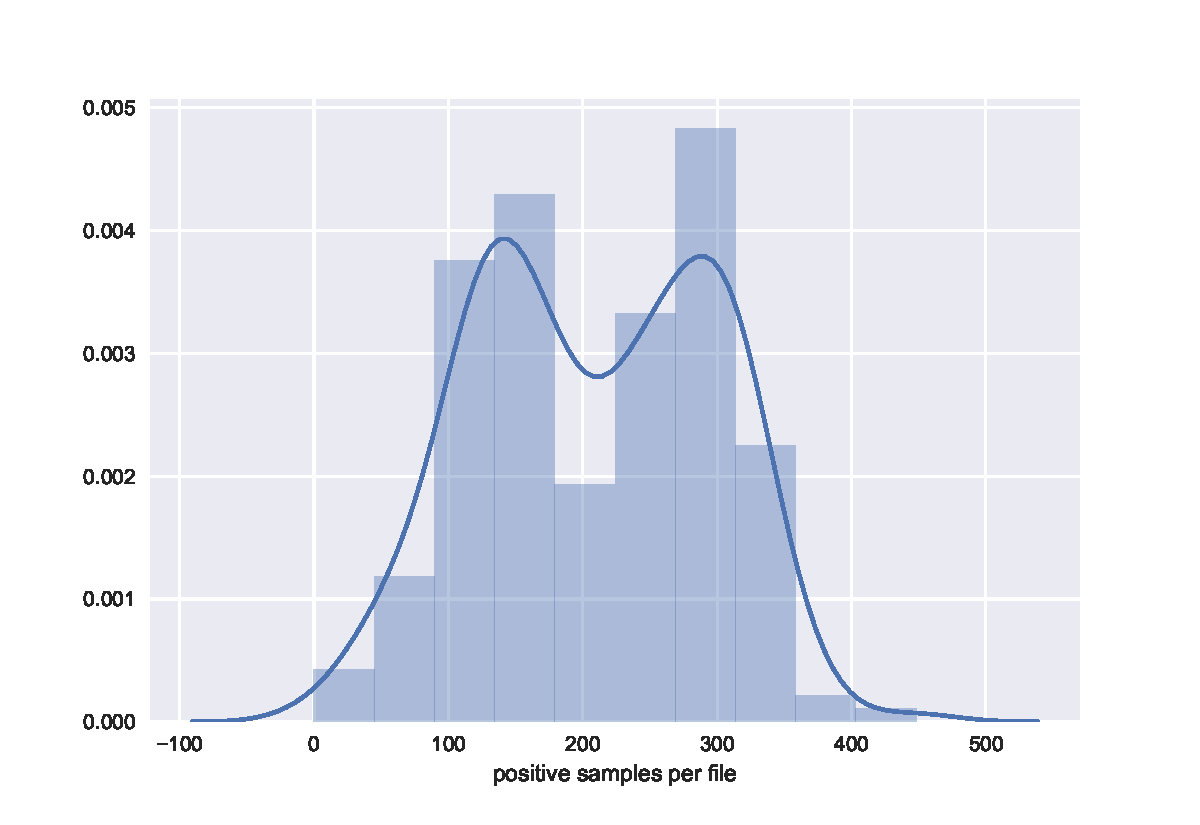
\includegraphics[width=\textwidth]{figures/distribution.pdf}
  \caption{Distribution of the number of positive samples per file}
  \label{fig:data_dist}
\end{figure}

%%% Local Variables:
%%% mode: latex
%%% TeX-master: "report"
%%% End: